\bookchapter{פרק 37: מהפכת הפרדיגמה — מ“לכתוב קוד” ל“לפקד על AI בכתיבת קוד”}

\chapterintro{ברכות! מי שפותח את הספר הזה עומד בדיוק בלב של מהפכת פרדיגמה מקצועית. נקודת הפתיחה של המהפכה הזאת הייתה משפט אחד שמתכנת פרסם ברשתות החברתיות ב-2025. נשמע קצת דרמטי? אבל כך זה בדיוק קרה.}

\booksection{א. הולדת ה-Vibe Coding: תנועה שנולדה ממשפט אחד}

בפברואר 2025, Andrej Karpathy — שימו לב לשם הזה, עוד נפגוש אותו כמה פעמים בהמשך — פרסם ברשתות החברתיות ציוץ שצוטט שוב ושוב: “יש דרך תכנות חדשה שנקראת Vibe Coding: נוהגים לגמרי לפי התחושות (vibes), מתעלמים מפרטי הקוד, ונותנים ל-AI לעשות הכול. אומרים מה שרואים, מעתיקים ומדביקים, ובעיקר — שיעבוד.”

ההתבטאות שנראתה כמו הערה אגבית העניקה בדיוק שם לתזוזת פרדיגמה שכבר התחוללה בשקט: בני האדם כבר לא כותבים קוד שורה-שורה, אלא מתארים כוונה בשפה טבעית, וה-AI מבצע. ניסוחו של Karpathy נושא גוון שובב, אבל מאחוריו מסתתרת תובנה עמוקה: כשיכולת יצירת הקוד של ה-AI חצתה סף מסוים, צוואר הבקבוק של התכנות כבר אינו “האם אני מסוגל לכתוב את השורה הזאת”, אלא “האם אני מבין לעומק מה בעצם אני רוצה”.

\begin{tcbinfo}{טיפ קטן: מה זה Vibe?}
מילולית, Vibe פירושו “אווירה, תחושה”. Vibe Coding הוא “לפקד על AI לתכנת לפי התחושות” — אתם מתארים מה אתם רוצים, וה-AI דואג ליישום. זכרו את המילה הזאת: היא תעודת הלידה של המהפכה הזאת.

\end{tcbinfo}

מאותו רגע המשמעות של המילה “קידוד” התפצלה: הקידוד המסורתי הוא תרגום עיצוב לתחביר; הקידוד החדש הוא תרגום כוונה להוראות. הראשון מאתגר את האצבעות, השני מאתגר את הראש.

המונח Vibe Coding מיהר להתגלגל מבדיחה גחמנית למושג הנדסי רציני. עד אמצע 2026 הוא כבר התפתח ממם אינטרנטי למתודולוגיה שלמה — המכסה את כל התהליך, מניסוח דרישות וניהול הקשר ועד אימות איטרטיבי והבטחת איכות. אנשים הבינו גם ש“ללכת לפי התחושות” הוא רק שלב ההתחלה, ושתכנות יעיל באמת בעזרת AI דורש שיטת חשיבה מסודרת. ושיטת החשיבה הזאת היא בדיוק מה שהספר הזה מעניק לכם.

\booksection{ב. המצב ב-2026: עידן ה-Agentic Engineering}

עד אוגוסט 2026 עבר עולם התכנות בעזרת AI כמה איטרציות פרדיגמה חשובות. Vibe Coding היה הניצוץ הראשוני, אבל במהרה התברר: כשמדברים עם ה-AI רק “לפי התחושות”, איכות הקוד שמתקבל אינה יציבה כלל — לפעמים מרשימה, לפעמים כישלון חרוץ. וכך הפרדיגמה החלה להתפתח: מתכנות שיחתי פשוט לעבר הנדסת Agent מובנית.

שוב Karpathy — בתחילת 2026 הוא טבע את המושג Agentic Engineering. בניגוד ל“אמרת — הופק” של Vibe Coding, Agentic Engineering מדגיש: נותנים ל-AI מטרה, והוא מתכנן בעצמו את הצעדים, קורא לכלים, מאמת תוצאות ומתקן באיטרציות. ה-AI אינו עוד מחולל קוד, אלא סוכן חכם (Agent) שמסוגל לחוש את הסביבה, לקבל החלטות ולבצע פעולות.

התזוזה הזאת הביאה לשלושה שינויים מכריעים:

\begin{enumerate}
  \item מצב האינטראקציה השתנה: מ"שאלה-תשובה" ל"קובעים מטרה ומעבירים את השליטה".
  \item התוצר של העבודה השתנה: מ"קטע קוד" ל"פרויקט שלם וממלא".
  \item תפקיד האדם השתנה: מ"סקירת קוד שורה-שורה" ל"הגדרת גבולות ואישור תוצאות".
\end{enumerate}

המספרים לא משקרים: בגרסת Cursor 3 שיצאה באפריל 2026, שיעור השימוש במצב Agent עקף לראשונה את מצב השלמת ה-Tab — סימן לכך שהמפתחים עברו בהמוניהם לאופן עבודה זה; ו-Claude Code, כלי התכנות בעזרת AI המקורי לטרמינל, הגיע עד אמצע 2026 להכנסה שנתית מואצת של 2.5 מיליארד דולר. גרף המגמות הבא ממחיש את רגע החצייה:

\begin{center}
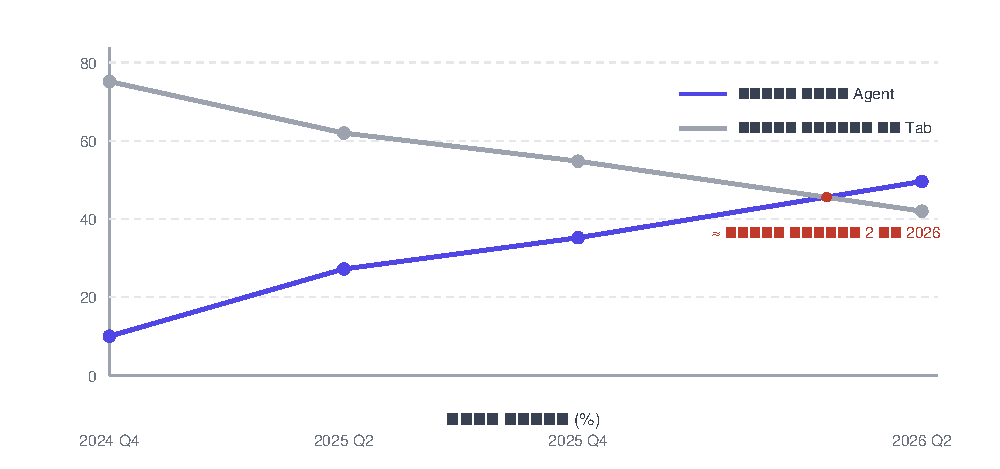
\includegraphics[width=0.92\linewidth]{figures/fig-di-san-shi-qi-zhang-1}
\\[2pt]\small איור 1: מגמת שיעור השימוש במצבי האינטראקציה של תכנות בעזרת AI (הערכה על סמך נתוני סקרי התעשייה; ברבעון השני של 2026 מצב Agent עקף את השלמת ה-Tab)
\end{center}

אבל בין כתלינו לאמת: השינויים בכלים ובמודלים הם רק החלק הנראה לעין. בין אם אתם עובדים עם Cursor ובין אם עם Claude Code, ובין אם המודל מאחורי הקלעים הוא GPT-5 או Claude 4.5 — כל מי שמצליח בתכנות בעזרת AI מציית לאותה מתודולוגיה בסיסית. וזה בדיוק מה שהמדריך הזה מלמד.

\booksection{ג. שינוי התפיסה המרכזי: מ-Coder ל-Conductor}

ההשכלה המסורתית לתכנות מלמדת אתכם להיות Coder — להבין תחביר, לשנן API ולנפות שגיאות לוגיקה. בעידן התכנות בעזרת AI התפקיד הזה מוגדר מחדש: אינכם חייבים עוד לכתוב כל שורת קוד במו ידיכם, אבל עליכם להיות “מנצח” (Conductor) — להגדיר את שדה הקרב, לקבוע את החוקים, לחלק משימות ולאשר תוצאות.

לב השינוי הזה אינו בשאלה “האם אתם יודעים לתכנת”, אלא “האם אתם יודעים לחשוב בבהירות מה רוצים לעשות”. מנצח מעולה אינו בהכרח החייל הטוב ביותר, אבל עליו להכיר היטב את מטרת הקרב, את השטח ואת פריסת הכוחות. באותו אופן, מי שמצטיין בתכנות בעזרת AI לא בהכרח שולט בכל פרטי התחביר של כל שפה, אבל עליו להכיר היטב את מטרת הפרויקט, את אילוצי הארכיטקטורה ואת תקני האיכות.

טבלה זו ראויה לקריאה כפולה — היא מסכמת את מלוא משמעותו של שינוי התפקיד הזה:

\begin{center}
\begin{tabularx}{\linewidth}{|X|X|X|}
\hline
\textbf{ממד} & \textbf{Coder מסורתי} & \textbf{מנצח AI (Conductor)} \tabularnewline
\hline
מיומנות הליבה & שינון תחביר, קריאות API, ניפוי שגיאות & הגדרת דרישות, ניהול הקשר, שיפוט ואישור תוצאות \tabularnewline
אופן העבודה & כתיבת קוד שורה-שורה & תיאור כוונה וסקירת התוצר \tabularnewline
שליטה באיכות & מה שכתבת בעצמך — אתה יודע בדיוק מה יש בו & אימות התוצר של ה-AI באמצעות בדיקות וסקירה \tabularnewline
דרישות הידע & שליטה עמוקה בשפה או בפריימוורק מסוים & הבנה רחבה של התמונה הטכנולוגית המלאה, הבנה עמוקה של הלוגיקה העסקית \tabularnewline
איפה צוואר הבקבוק & מהירות הקידוד ושינון התחביר & בהירות החשיבה ויכולת הביטוי \tabularnewline
מקור השגיאות & שגיאות תחביר, השמטות לוגיות & דרישות מעורפלות, הקשר חסר \tabularnewline
\hline
\end{tabularx}
\end{center}

\begin{center}\small\color{gray}השוואת ממדי היכולת בין Coder מסורתי לבין מנצח AI\end{center}

אין זה אומר בשום פנים שידע בתכנות איבד מחשיבותו. דווקא ההפך: רק כשאתם מבינים את הקוד שה-AI כותב, אתם יכולים לסקור ולתקן אותו ביעילות; רק כשאתם מכירים מבני נתונים ואלגוריתמים, אתם יכולים לשפוט אם הפתרון שה-AI הציע הגיוני. מלאי הידע קובע את “תקרת הפיקוד” שלכם — אבל תפקיד הידע השתנה מ“כלי ביצוע” ל“בסיס לשיפוט”.

\booksection{ד. מדוע המתודולוגיה חשובה יותר מהכלים}

כלים מתחדשים כל שלושה חודשים, ומתודולוגיה מתפתחת רק כל שלוש שנים. ללמוד להפעיל כלי עלול להתיישן בעוד שלושה חודשים; לשלוט בדרך חשיבה יישאר רלוונטי גם בעוד שלוש שנים.

רבים שנכנסים לעולם התכנות בעזרת AI פותחים בשאלות “איזה כלי הכי טוב” ו“איזה מודל הכי חזק”. שאלות אלה אינן חסרות חשיבות, אבל הן שואלות את סדר העדיפויות בצורה שגויה. מפת הכלים באוגוסט 2026 שונה לחלוטין מזו של אוגוסט 2025 — Trae, Qoder וכלים נוספים עלו וירדו, Cursor התפתח מתוסף ל-IDE עצמאי ואז ל-Cursor 3, ו-Claude Code עבר מפרויקט ניסיוני לבחירה המרכזית לתכנות בטרמינל. אבל מאחורי התנודתיות הזאת, עקרונות החשיבה שעליהם נשענים המצליחים כמעט ולא השתנו.

מסיבה זו הספר הזה לא יבזבז עמודים על הוראת הפעולות הספציפיות של כלי מסוים — תוכן כזה מתיישן כשכותבים אותו. במקום זאת, כל משקלו של הספר מושם על מתודולוגיית חשיבה מוכחת: איך חושבים על דרישות, איך מתקשרים עם AI, איך מאמתים תוצרים ואיך ממשיכים לשפר. מי ששולט במתודולוגיה הזאת יסתגל במהירות לכל כלי; מי שלמד רק את פעולות הכלי מתחיל מאפס בכל החלפת כלי.

\begin{tcbinfo}{כדור הרגעה לקוראים שמתחילים מאפס}
אם אתם מתחילים מאפס, אל תיבהלו מהמילה “מתודולוגיה”. מתודולוגיה אינה פילוסופיה מופשטת; היא פשוט חוברת הפעלה של “איך חושבים כשנתקלים בבעיה”. זה כמו ללמוד לבשל: אפשר ללכת לפי מתכון צעד-צעד (הפעלת הכלי), אבל שף אמיתי מבין “למה מתבלים כך” ו“איך שולטים בעוצמת האש” (מתודולוגיה). הספר הזה יתחיל מהמושגים הבסיסיים ביותר, וכל עקרון ילווה בדוגמאות השוואה קונקרטיות, כדי שתבינו לא רק “מה” אלא גם “איך”.

\end{tcbinfo}

\begin{tcbpractice}{תרגול מעשי: צלמו "תמונת תפקיד" של עצמכם היום}
קחו דף ורשמו תשובות לשלוש שאלות: (1) איך אתם משתמשים היום ב-AI כדי שיכתוב קוד בשבילכם (אם בכלל השתמשתם)? (2) אתם דומים יותר ל-“Coder” מהטבלה או ל“מנצח”? (3) איך הייתם רוצים שאתם של בעוד שלושה חודשים יתארו את דרך העבודה שלכם? בסיום תקפלו את הדף בין דפי הספר, ותחזרו לקרוא אותו אחרי פרק 47 — תגלו שהשינוי מגיע מהר יותר משדמיינתם.

\end{tcbpractice}

\begin{tcbsummary}{סיכום הפרק}
\begin{itemize}
  \item ב-2025 Karpathy נתן למהפכת התכנות בעזרת AI את שמה — "Vibe Coding": מכתיבה שורה-שורה לתיאור כוונות בשפה טבעית
  \item ב-2026 התפתחות ל-Agentic Engineering: נותנים מטרה, מעבירים סמכות, ה-AI מתכנן ומבצע בעצמו, והאדם מאשר את התוצאות
  \item ב-Cursor 3 שיעור השימוש במצב Agent עקף לראשונה את השלמת ה-Tab; ההכנסה השנתית של Claude Code הגיעה ל-2.5 מיליארד דולר
  \item התפקיד החדש שלכם הוא Conductor (מנצח): להגדיר את שדה הקרב, לקבוע את החוקים, לחלק משימות ולאשר את התוצאות
  \item הכלים מתחדשים כל שלושה חודשים, המתודולוגיה מתפתחת רק כל שלוש שנים — למדו מתודולוגיה, לא פעולות
\end{itemize}

\end{tcbsummary}
